\chapter{Preliminaries}
\label{chp:preliminaries}

The design requirements for the robot is explained based on minimal required capabilities in Section \ref{sec:pre_design_requirements}.
Section \ref{sec:pre_energy_source_selection} evaluates two sources for energy harvesting and in Section \ref{sec:pre_locomotion_selection} two types of locomotion for the transiently powered robot are evaluated.
%Finally in Section \ref{sec:pre_transient_model}, a simple model will capture the relation between power harvested and distance covered by the robot.

\section{Design requirements}
\label{sec:pre_design_requirements}

This section explains the main areas considered while designing the battery-less transiently-powered robot.

\begin{enumerate}
	\item \textbf{Power}: 
	The robot should not rely on batteries.
	Energy can be harvested from ambient sources and stored in a supercapacitor. 
	Energy harvested in a controlled environment should charge the capacitor in under 10 seconds and stored energy should provide at least an operation time of 1 second i.e. a minimal 10\% power duty cycle.
	
	\item \textbf{Small form factor}: 
	The size and weight of the robot needs to be kept to a minimum, reducing the energy required for movement.
	Additionally, designing the robot to use low cost off-the-shelf parts makes it convenient to build collectives of small transiently-powered robots.
	
	\item \textbf{Locomotion}:
	An efficient locomotion type needs to be selected for the movement on flat surfaces, to optimize the distance that can be covered with a single capacitor charge.
	%Movement will consume the largest amount of energy from the total available energy budget.

	\item \textbf{Autonomous navigation}:
	Despite the frequent power failures, the transiently-powered robot needs to be able to complete a movement with an acceptable error when compared to its battery powered counterpart.
\end{enumerate}

\section{Energy Source Selection}
\label{sec:pre_energy_source_selection}
% RF harvesting seems prommesing
% Wispcam requires approx 4 seconds to harvest 20mJ at a distance of 20cm from the reader \cite{naderiparizi_rfid_2015}
% better to only use RF for communication and harvest energy from another source \cite{konstantioulos}

In this section two sources for the harvesting of ambient energy are evaluated: radio signals and solar.
The charge times of an energy storage element are measured for a variety of distances from the selected sources.

%The average input power is defined as

%\begin{equation}
%	P_{\text{in}} = \frac{E_{\text{cap}}}{t_{\text{charge}}},
%\end{equation}

%\noindent
%where $E_{\text{cap}}$ the energy stored in a capacitor and $t_{\text{charge}}$ the average charge time.
%The energy stored in a capacitor given minimum and maximum voltage levels is defined as

%\begin{equation}
%\label{eqn:energy_cap}
%	E_{\text{cap}} = \frac{1}{2}C(V_{\max} - V_{\min})^{2},
%\end{equation}

%\noindent
%where $C$ is the capacity of a the capacitor, $V_{\min}$ is the minimum and $V_{\max}$ is the maximum voltage level of a capacitor.

\subsection{Energy Harvesting and Storage}
\label{sec:pre_energy_harvesting_storage}
Energy is harvested using a Texas Instruments BQ25570 energy harvester~\cite{bq25570_2017}, which includes a nanopower boost charger with maximum power point tracking to extract the optimal amount of energy. 
The harvested energy is stored in a 22\,mF - 4.5\,V supercapacitor from AVX~\cite{avx_bestcap_2017}, chosen for its low leakage current and small size.
The BQ25570 comes with a buck converter to efficiently regulate the capacitors voltage down to the system voltage of 2.2\,V.
External resistors are used to program voltage thresholds, allowing to automatically enable and disable the buck converter based on minimum and maximum thresholds.
The minimum threshold is set to 2.2\,V and the maximum threshold is set to 4.2\,V.
%Using (\ref{eqn:energy_cap}) the energy stored in the capacitor is equal to

%\begin{equation}
%\label{eq:cap2}
%E_{\text{cap}} = \frac{1}{2} 0.022 (4.4 - 2.2)^2 = 53.24 \text{\,mJ}.
%\end{equation}

%Additionally the resistors are used to set the overvoltage protection and the buck converter output voltage.
%The minimal supply voltage is determined by the component with the highest minimal voltage requirement, in this case 2.0\,V.
%To make sure that a small drop in system voltage would not create instability a margin of 0.2\,V was added, resulting of a system voltage of 2.2\,V.

\subsection{Measuring the Charge Time}

The buck converter of the energy harvester is automatically enabled when the maximum voltage threshold is reached.
A load is connected to the output of the buck converter to quickly drain the energy from the capacitor.
In this case load is chosen such that the power consumed by the load $P_{\text{load}} \gg P_{\text{in}}$, the harvested input power .
By connecting a Saleae logic analyzer~\cite{saleae_2017} to the output of the buck converter, the off time of the power cycles can be recorded.
The time that the output of the buck converter is disabled is equal to the time to charge the capacitor from the minimum to the maximum threshold.

\subsection{Energy Harvesting from radio signals}

\subsubsection{Harvesting using a WISP}
To be able to connect an external harvester, a WISP 5~\cite{sample_transim_2008} is modified.
The integrated energy harvester, the storage capacitor and the diode to bypass the harvester, are removed from the WISP.
A wire is soldered to the input pin pad of the removed harvester on the WISP PCB.
This wire is connected directly to the input of the external energy harvester.

\subsubsection{Measurements}
Energy is provided to the WISP using a Impinj Speedway R1000 RFID reader~\cite{impinj_eol_2017, indy_r1000_2017}.
This reader is connected to a Laird S90028PCR antenna~\cite{laird_s9028pcr_2017}.
The WISP is positioned 25, 35 and 45\,cm away from the reader and the charge times are recorded.

\begin{table}[t]
	\centering
	\caption{The average charge time by harvesting energy from RFID transmitter.}
	\label{tab:res_rf_harvest}
	\begin{tabular}{|l||l|l|l|}
		\hline
		Distance from RFID reader (cm) & 25 & 35 & 45 \\
		\hline \hline
		Average charge time (s) & 49.1 & 61.1 & 164.8 \\
		%Average input power & 1.086\,mW & 0.871\,mW & 0.323\,mW \\
		\hline
	\end{tabular}
\end{table}

\subsubsection{Results}
The time to charge the capacitor is more than 49\,s, see Table \ref{tab:res_rf_harvest}.
As the WISP is placed further away from the reader the charge times increase significantly.
While the distance increases the harvested power is decreased due to path loss and reflections of the signal.

\subsection{Energy Harvesting from Light}
Sunlight is not always available or strong enough to charge the robots supercapacitor in acceptable time.
Alternatively, lamps can provide uniform light to the area where the robot moves around.
In this section the capacitor charge time is evaluated for different solar panel and light source combinations.
To accurately measure the power that is harvested from each solar panel, their performance was evaluated in a darkroom at TU Delft Embedded Software Lab.

\subsubsection{Solar panels}
Three solar panels are tested, each different in material, efficiency and panel size, as seen from Table \ref{tab:solar_panels}.

\begin{table}[t]
	\centering
	\caption{Specification of the three solar panels tested in the experiment.}
	\label{tab:solar_panels}
	\resizebox{\columnwidth}{!}{%
		\begin{threeparttable}
			\begin{tabular}{|l|l|l|l|}
				\hline
				& Material & Efficiency (\%) & Dimensions (mm) \\
				\hline \hline
				Banggood~\cite{bangood_solar_2017}& Poly-Si & 17 & 40x30 \\
				INYS SLMD121H04L-ND~\cite{ixolar_slmd121h04l_2017}\textsuperscript{1}& Mono-Si & 22 & 43x34 \\
				Azurspace 3G28C~\cite{azurspace_3g28c_2017}& Triple Junction GaAs& 28 & 80x40 \\
				\hline
			\end{tabular}
			\begin{tablenotes}
				\small
				\item [1] Two panels in parallel
			\end{tablenotes}
		\end{threeparttable}
	}
\end{table}


\subsubsection{Lamps}
Low cost solar simulators can for example consist of a combination of LED and halogen light bulbs to simulate sunlight and are used to test the performance of solar panels~\cite{grandi_tia_2014}.
However, the goal is to have a controlled uniform lighting environment where the robots have roughly constant charge times.
Solar panels do not only harvest energy from the visual light spectrum but harvest at least as much from the infrared light spectrum, therefore not only light but also heat shortens the charge time~\cite{ixolar_slmd121h04l_2017}.
Halogen lamps have a lower color temperature than the sun, but also emit waves far into the infrared spectrum.
The light sources used in this experiment are a 60\,W halogen bulb, a 120\,W halogen bulb and two 150\,W Philips  BR125, infrared (IR) incandescent reflector lamps~\cite{philips_irlamp_2017} where one is translucent and the other uses a red filter.

\subsubsection{Measurements}
Three charge time measurements are performed, each lamp is positioned 10\,cm, 30\,cm and 50\,cm from the solar panels.
As reference, the charge times are also measured on a sunny November afternoon, inside the office room of TU Delft Embedded Software lab. 
% Additionally, for these three distance the temperature was measured at the solar panel using a K-type thermocouple supplied with an Extech EX330 multimeter and the light intensity using the luxmeter on a MASTECH MS8229 multimeter.

\subsubsection{Results}
% No difference between the heatlamps in power consumed
% Halogen distributes the light more even
% Panel from nuna
% Refer to appendix for temperature and light data?

The results obtained from the measurements show a non-linear relation between the charge times and the distance between the solar panel and the source, as seen in Table \ref{tab:light_results}.
Increasing the output power of the source and decreasing the distance between panel and the source, both decrease the charge times.
However, there is no obvious best performing combination of solar panel/light source.

Note that with some lamps a shadowing pattern is observed due to the construction of the lamps.
The 60\,W and 150\,W IR lamps have a spherical design, and their construction creates an uneven circular shadowing pattern. 
This becomes more significant on larger distances.
The 120\,W halogen lamp has a tubular design and in combination with the light fixture most of the light is reflected down with minimal shadowing of the lamp resulting in a more even light distribution.
Therefore, it is chosen to provide light in the controlled setup where the robots can move around with roughly constant charge times.
For the 120\,W halogen lamp at the distances 30\,cm and 50\,cm the INYS solar panel seems to perform the best.

Additionally, the charge times were recorded during a sunny 30 minute time slot (2:30--3:00\,PM, 23 November 2017) for each solar panels, as seen in Table \ref{tab:solar_results}.
The Azurspace solar panel has the shortest supercapacitor charge time, this can be expected because the triple junction allows it to harvest energy from the broadest part of the light spectrum.

%Both the temperature and illumination increase by decreasing the distance between the light source and the solar panel. 
%Secondly, increasing the output power of the lamp increases temperature and illumination as well. 

\begin{table}[t]
	\centering
	\begin{threeparttable}
		\caption{The average supercapacitor charge times, for each panel at three distances from the sources.}
		\label{tab:light_results}
		\begin{tabular}{|l|l||l|l|l|l|}
			\hline
			\multirow{2}{*}{Distance (cm)} & \multirow{2}{*}{Panel} & \multicolumn{4}{c|}{Average charge time per source (s)} \\
			%\hline
			& & 60\,W & 120\,W & 150\,W clear & 150\,W red \\
			\hline \hline
			\multirow{3}{*}{10} & Banggood& 3.08 & 2.19 & 0.99 & 0.73 \\
			& INYS & 2.52 & 0.75 & 0.46 & 0.51 \\
			& Azurspace & 5.62 & 3.22 & 1.55 & 3.54 \\
			\hline
			\multirow{3}{*}{30} & Banggood & 6.45 & 6.72 & 7.83 & 1.88 \\
			& INYS & 8.00 & 5.68 & 2.67 & 1.50 \\
			& Azurspace & 23.05 & 8.25 & 19.75 & 20.33\\
			\hline
			\multirow{3}{*}{50} & Banggood & 26.28 & 17.59 & 17.91 & 9.46 \\
			& INYS & 45.41 & 15.53 & 9.28 & 6.97 \\
			& Azurspace & 106.67 & 24.18 & 46.20 & 93.91 \\
			\hline
		\end{tabular}
		\begin{tablenotes}
			\small
			\item The charge times are normalized to a panel dimension of 40$\times$40 mm.
		\end{tablenotes}
	\end{threeparttable}
\end{table}

\begin{table}[t]
	\centering
	\caption{The average charge time harvesting ambient light during a sunny afternoon.}
	\label{tab:solar_results}
	\begin{tabular}{|l|l|}
		\hline
		Panel & Charge time (s) \\
		\hline \hline
		Banggood & 3.84\\
		INYS & 3.55\\ 
		Azurspace & 2.81\\
		\hline
	\end{tabular}
\end{table}

\subsection{Conclusion}

The results from RF experiments show that the minimum charge time is 49\,s, which more than doubles with only a 20\,cm distance increase from the reader.
%The mobility of the robot results in widely varying charge times and possible dead spots where the robot is not able to receive any power.
Light is more readily available and by illuminating the area where the robot moves around with a 120\,W halogen lamp source, 6\,s charge times can be achieved when the light is positioned at a distance of 30\,cm from the solar panel.
With the solar panel eight times shorter charge times can be achieved, and therefore solar is chosen to be the energy source for the transiently powered robot.

\begin{figure}[!ht]
	\centering
	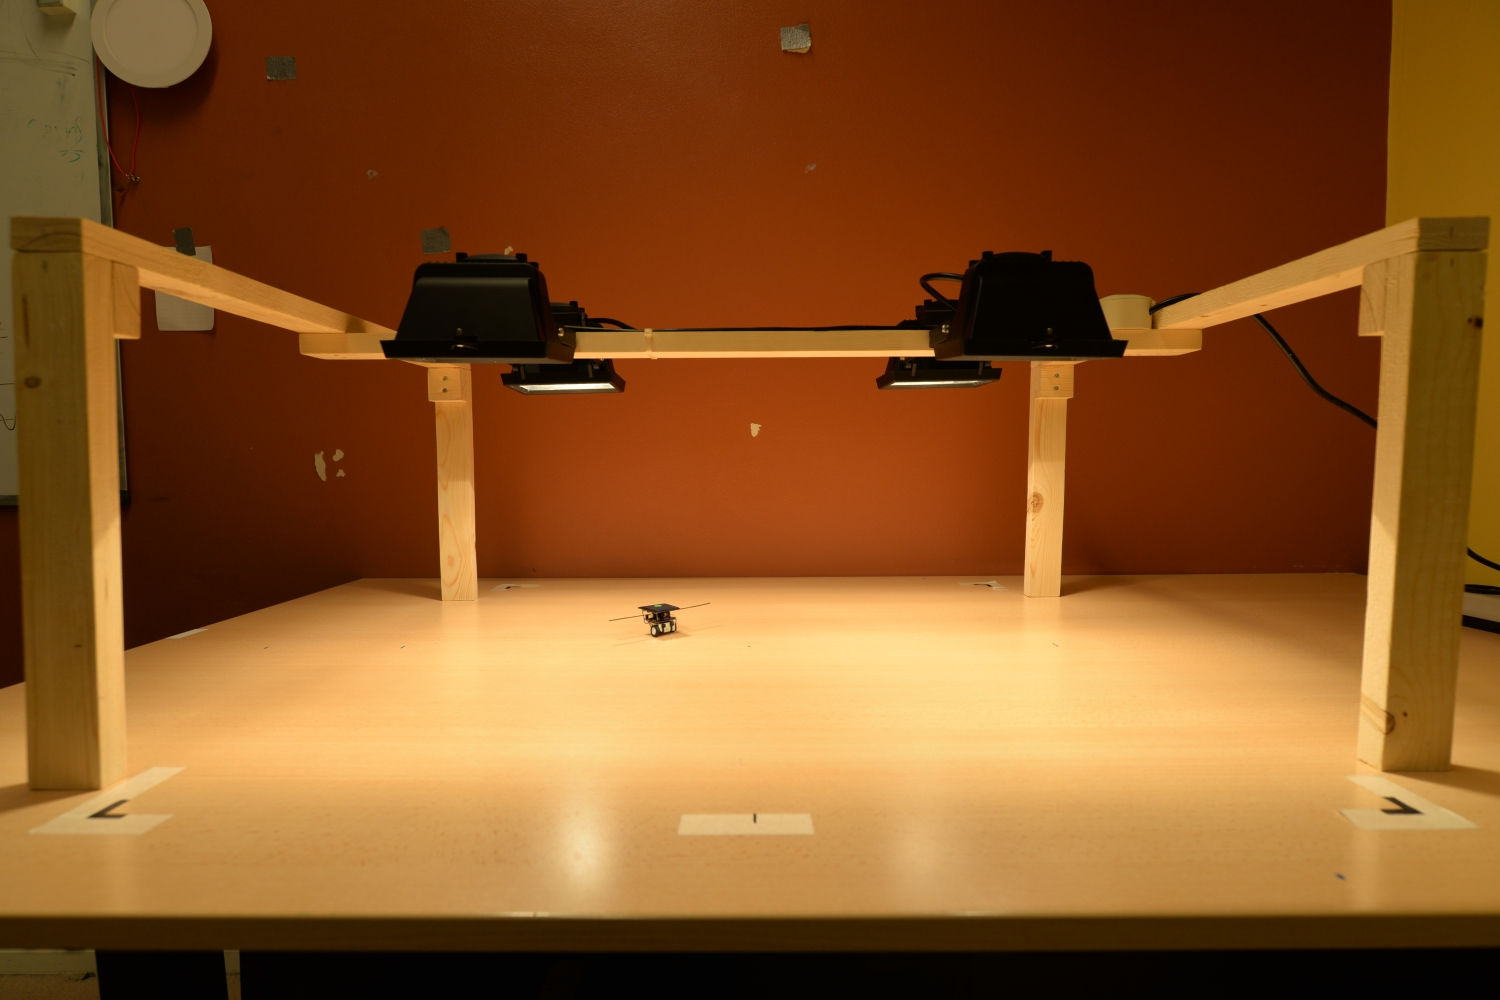
\includegraphics[width=0.8\textwidth]{pics/light_setup.jpg}
	\caption{The light setup consisting out of four halogen lamps placed 30\,cm from the table top, providing energy to the robot.}
	\label{fig:light_setup}
\end{figure}

\subsection{Light setup}

To create an area where the transiently-powered robots can move around with approximately constant charge times, a light setup is created using wooden beams, as shown in Figure \ref{fig:light_setup}.
Mounted in this frame are four 120\,W halogen lamps, previously determined to provide the most uniform light distribution and short charge times.
The frame spans an area of 95$\times$66 cm and distances the lamps 30\,cm from the tabletop.

\section{Locomotion Selection}
\label{sec:pre_locomotion_selection}

Wheeled locomotion types are assumed to be the most efficient on flat surfaces.
Therefore, in this section two wheeled locomotion types are evaluated: the stepper motor and the DC motor.
The robot can navigate without external feedback from one location to another, but accurate locomotion and basic odometry are required.

\subsection{Stepper motor-based Locomotion}

The GRITSBot~\cite{pickem_icra_2015} uses stepper motor based locomotion which already include basic odometry, as described in Section \ref{sec:rw_locomotion}.
The upcoming section further investigates the use of stepper motor based locomotion for a transiently-powered robot.

\subsubsection{Operation of a Stepper Motor}
Stepper motors are permanent magnet DC motors that start to rotate by supplying current to the motor coils in a specific direction.
The bipolar stepper motor used, requires current to be pulsed trough each of the four connections, in a fixed pattern, in order to rotate it forwards or backwards.
A Microcontroller (MCU) is used to keep track and control stepper motor position from a sequence of four.
The outputs of the MCU cannot supply enough current to drive a bipolar stepper motor, therefore a dual H-bridge is required to control the current trough each coil.

%TODO make new schematic stepper figure!
%http://homemaderobo.blogspot.nl/2012/03/stepper-motor.htm
%\begin{figure}
%	\centering
%	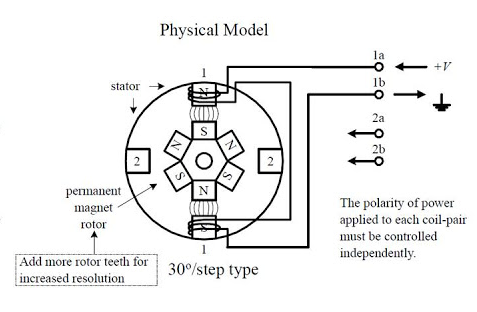
\includegraphics[width=\textwidth]{pics/bipolar_stepper.png}
%	\caption{Need better / simpler figure here!}
%	\label{fig:bipolarstepper}
%\end{figure}

%\subsubsection{Current Consumption}
%TODO values that calculate the current per motor?
%TODO ADD CURRENT MEASUREMENTS @ 2.2 v
%The current consumed by a stepper motor is constant and independent of the angular velocity of the rotor.
%The average current consumed is equal to: $\textrm{I} = V_{\text{supply}}/R_{\text{coil}}$.
%Therefore, running the motor at maximum speed translates the most electrical energy into kinetic energy.
%However, the motor speed is inversely proportional to the output torque of the motor and the maximum speed is limited by the minimal required output torque.
%The current trough the coils is constant, so the faster the stepper motor changes step the more energy can be transformed into movement.
%Increasing the rotational speed of the stepper motor decreases the torque output of the motor.
%Therefore the speed is limited by the amount of torque required to perform the movement.

\subsubsection{Control and Rotor Synchronization}

The only way to guarantee that the rotor stays aligned with the coil, is to keep the coil energized until the next position is instructed and the succeeding coil is energized. 
On the first startup the rotor may not be aligned with the last position in the sequence of four.
As a result an error between one and three steps can occur before the energized coil and rotor are synchronized.

In case the stepper motor is rotating and the power is removed, misalignment between the rotor and the last energized coil can occur. While the rotor could be moving from one position to the next, it has not moved at all (undershoot) or can continue to move to the next position due to inertia of the rotating mass (overshoot). 
To determine what would be more likely, undershooting or overshooting, the following experiment has been performed to determine the error in the number of steps.

\subsubsection{Experimental setup}

The motor used for this experiment is a 6\,mm permanent magnet bipolar stepper motor from Nidec~\cite{nidec_stepper_2017}.
For this motor one rotation is equal to 20 steps i.e. five times the sequence of four.
This stepper motor is suspended and a needle glued to the motor shaft. The needle rotates over a round piece of paper which is divided by markings in 20 steps. %, as seen from Figure \ref{fig:step_counting}.
First the rotor and coil are synchronized by moving four steps, and the position of the needle is visually recorded and written down. 
Then the stepper motor is commanded to make one rotation equal to 20 steps. 
After rotating 20 steps the power is removed from the coils and the needle position is again visually recorded and written down.

\begin{figure}
	\centering
	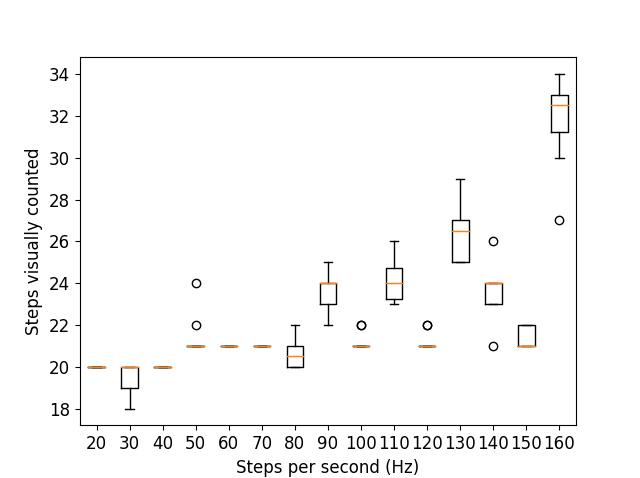
\includegraphics[width=0.8\textwidth]{pics/figure_intertia.png}
	\caption{The visually counted number of steps when power is removed after 20 steps. The stepper motor is likely to overshoot and this effect becomes more significant with increased step frequency.}
	\label{fig:step_results}
\end{figure}


%\begin{subfigure}[b]{0.38\textwidth}
%	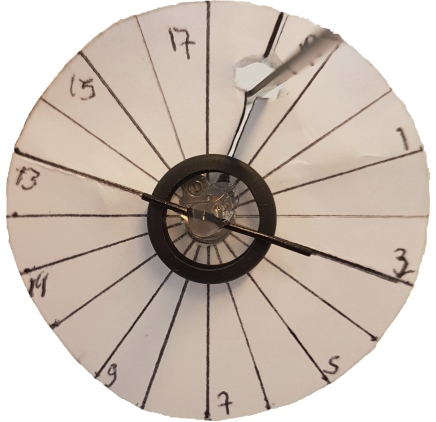
\includegraphics[width=\textwidth]{pics/step_counting.jpg}
%	\caption{Experimental setup for determining error in the number of counted steps}
%	\label{fig:step_counting}
%\end{subfigure}	


\subsubsection{Stepper Motor Inertia Result}

Figure \ref{fig:step_results} shows the result of the experiment.
The stepper motor on average overshoots, i.e. does more steps than commanded when the power is removed.
This effect becomes more significant with increased step frequency.
While this experiment only shows the effect for an unloaded motor, it is likely that a synchronization error also occurs when a transiently-powered robot would be powered using two stepper motors in differential drive.
After every power interrupt, the rotor of each motor needs to be synchronized with the energized coil by the MCU.
As a result the robot could make a random turn if the error between the motors is not equal.

\subsection{DC Motor locomotion}
\label{sec:pre_dc_motor_locomotion}
Small DC motors are commonly selected to provide locomotion for small robotic platforms as seen from Table \ref{tab:comparison_robot_platforms}.
In this section the DC motor is evaluated as the locomotion type for the transiently-powered robot.

\subsubsection{Operation of a DC Motor}

When voltage is applied to the motor, current rises as quickly as the inductance in the motor windings allows.
DC motors produce an initial startup peak because the back electromotive force (back EMF) is initially zero.
The current reaches a maximum when the rotor starts to rotate and a back EMF is generated.
The back EMF increases further while the motor accelerates to its steady state speed, and the speed is determined by the voltage supplied.

If a load is applied to the DC motor, the current consumed by the motor is increased because current is proportional to the torque applied to the motor.
Additionally, the angular velocity of the motor decreases while the torque is inversely proportional to the angular velocity of the motor.

\subsubsection{Evaluation of the Start Current Peak}
The DC motors used for robots are normally powered directly from the battery since linear or switch-mode power regulators are not able to supply the high start currents.
%In the worst case the start current peak can be equal to the stall current of the motor.
However, the use of a supercapacitor requires a regulator to make efficient use of the energy stored, as described in Section \ref{sec:pre_energy_harvesting_storage}.
The switch-mode regulator that is part of the BQ25570 energy harvester is only able to supply a peak output current of 110\,mA~\cite{bq25570_2017}.

%To evaluate the magnitude of the current peak, the free running current profile of 
The 206-11 DC motor from Precision Microdrives~\cite{gearmotor_206-110_2017} is the selected to be evaluated.
From the datasheet a typical start current of 185\,mA can be found for its rated operating voltage of 3\,V.
However, the system voltage chosen for transiently-powered robot is 2.2\,V.
To determine the startup current of a 206-110 motor when supplied with 2.2\,V, a two second current trace is recorded using a Monsoon Power Monitor~\cite{monsoon_powermonitor_2017}.

The maximum current measurements for three different motors is shown in Figure \ref{fig:free_running_current}.
The results show that a supply voltage of 2.2\,V reduces the start current peak to 140\,mA.
This is still above 110\,mA and the robot needs to power two motors in a differential drive configuration to allow steering.

A solution is to use Pulse Width Modulation (PWM) to reduce the motor speed and average current consumption.
Combining PWM with a large bulk capacitor should enable the buck converter to start the motors.
However, the duty cycle is limited to a maximum of $100/(2\times140/110) \approx 39\%$, and is further reduced by the load applied to the motors as a result of the robots own weight.

\begin{figure}%[h!]
	\centering
	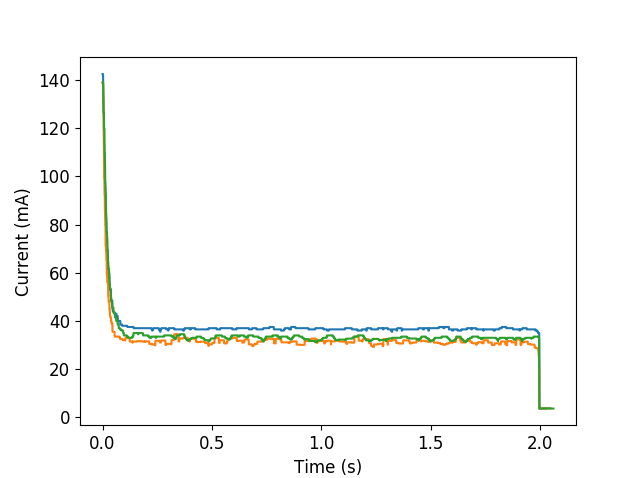
\includegraphics[width=0.8\textwidth]{pics/free_running_current.png}
	\caption{The free-running current profile of three 206-110 dc motors supplied with 2.2\,V. Dc motors have a startup current peak significantly higher that their steady state current.}
	\label{fig:free_running_current}
\end{figure}

\subsection{Conclusion}
%Stepper motor have a lower efficiency than normal dc motors because a constant current is consumed.
The only way the rotor and stator of a stepper motor aligned is by keeping the stepper motor coil energized.
Frequent power interrupts could lead to loss of synchronization between the energized coil and position of the rotor as a result of rotor inertia.
The error due to inertia becomes more significant with increase rotational speed.
Loss of synchronization can result in random behavior of a differential drive robot, as one stepper motor may require a different amount of steps before synchronization than the other.

Normal DC motors have a high start current which the buck converter from the harvester might not be able to supply.
PWM can be used to reduce the average current consumed by the motor and a large bulk capacitor can supply short high current demand from the motors.
The DC motor is chosen as the locomotion type used for the transiently-powered robot.
